\documentclass{beamer}

\usepackage[utf8]{inputenc}
\usepackage{color, xcolor}

% \usepackage[hidelinks]{hyperref}[citecolor=green]
% \usepackage{cite}
% \usepackage{appendix}

\usepackage{multicol}
\usepackage{fancyhdr}
\usepackage{listings}
\usepackage{graphicx, subfig}
\usepackage{float}
\usepackage{enumerate}

\usepackage{amsfonts}
\usepackage{eucal}
\usepackage{amsmath}
\usepackage{amssymb}
\usepackage{gensymb}
\usepackage{amsthm}
\usepackage{makecell}
\usepackage[ruled]{algorithm2e}
\usepackage{tikz}
\usetikzlibrary{positioning}

\usepackage[backend=bibtex,style=authoryear]{biblatex}
\bibliography{reference.bib}
\setbeamerfont{footnote}{size=\tiny}
\renewcommand{\thefootnote}{[\arabic{footnote}]}

\title{Explore the Influence of Words on Stock Volatility and the Most Important Word Features \\ --- Based On 10-K report
}
\author{
  \parbox{0.3\textwidth}{
    \centering WANG Zeyu
    \vspace{.25cm}
  }
  \parbox{0.3\textwidth}{
    \centering LIU Chang
    \vspace{.25cm}
  }
  \parbox{0.3\textwidth}{
    \centering TAN Huangao
    \vspace{.25cm}
  }
  \parbox{0.3\textwidth}{
    \centering LI Borui
  }
  \parbox{0.3\textwidth}{
    \centering ZHU Xinqi
  }
  \parbox{0.3\textwidth}{
    \centering GAO Yifeng
  }
}
\date{\today}

\usetheme{Madrid}
\usecolortheme{default}
\setbeamertemplate{navigation symbols}{}

\setbeamertemplate{footline}
{
  \leavevmode%
  \hbox{%
  \begin{beamercolorbox}[wd=0.5\paperwidth,ht=2.25ex,dp=1ex,center]{author in head/foot}%
    \usebeamerfont{author in head/foot}\insertsection
  \end{beamercolorbox}%
  % \begin{beamercolorbox}[wd=.4\paperwidth,ht=2.25ex,dp=1ex,center]{title in head/foot}%
  %   \usebeamerfont{title in head/foot}\inserttitle
  % \end{beamercolorbox}%
  \begin{beamercolorbox}[wd=0.5\paperwidth,ht=2.25ex,dp=1ex,center]{date in head/foot}%
    \usebeamerfont{date in head/foot}\insertshortdate{}\hspace*{2em}
    \insertframenumber{} / \inserttotalframenumber\hspace*{2ex}
  \end{beamercolorbox}}%
  \vskip0pt%
}

\usefonttheme[onlymath]{serif}

\begin{document}

\section*{Cover}
\frame{\titlepage}

\section*{Contents}
\begin{frame}{Contents}
  \tableofcontents
\end{frame}

\section{Introduction}

\begin{frame}{Introduction - Goals}

  Our project aims to: \vspace{.25cm}
  \begin{itemize}
    \item Predict the log volatility of the following year via the MD\&A section of the Form 10-K; \vspace{.25cm}
    \item Find out the importance of each token and check whether they are similar over the years.
  \end{itemize}

\end{frame}

\begin{frame}{Introduction - Motivation}

  These two goals are meaningful because: \vspace{.25cm}

  \begin{itemize}
    \item The MD\&A section is most related to the forecasting in Form 10-K; \vspace{.25cm}
    \item A better predicting model can lead to a better portfolio; \vspace{.25cm}
    \item Such models show the market information transmission mechanisms. \vspace{.25cm}
  \end{itemize}

\end{frame}

\begin{frame}{Introduction - Dataset}

  We use a portion of the data in 10-K Corpus \footfullcite{kogan2009predicting}, including: \vspace{.25cm}

  \begin{itemize}
    \item The tokenized MD\&A sections;
          \begin{itemize}
            \item[-] (e.g. 1996.tok.tgz) \vspace{.25cm}
          \end{itemize}
    \item The log volatility in the related year.
          \begin{itemize}
            \item[-] (e.g. 1996.logvol.-12.txt, 1996.logvol.+12.txt) \vspace{.25cm}
          \end{itemize}
  \end{itemize}

\end{frame}

\section{Methods}

\begin{frame}{Methods - Lemmatization, Stemming and Stop token filter}

  We use the Natural Language Toolkit (NLTK) \footfullcite{nltk-py} for lemmatizer, stemmer and stop token filter. \vspace{.25cm}

  \begin{itemize}
    \item Some words are regarded as insignificant in text analysis;
          \begin{itemize}
            \item[-] (e.g. a, an, the, above, across) \vspace{.25cm}
          \end{itemize}
    \item Words appear in several inflected forms but with same meaning should be considered as the same;
          \begin{itemize}
            \item[-] (e.g. {achieves, achieved, achievement, achievement} $\rightarrow$ achiev) \vspace{.25cm}
          \end{itemize}
  \end{itemize}

\end{frame}

\begin{frame}{Methods - Term Frequency–Inverse Document Frequency (TF-IDF)}

  The term frequency–inverse focument frequency (TF-IDF) \footfullcite{sparck1972statistical} \footfullcite{robertson2004understanding} measures the importance of a word to a document in corpus via: \vspace{.25cm}

  $$
    \begin{aligned}
       & \text{(Term frequency)}             & \mathrm{tf}(t, d)  & = \frac{f_{t, d}}{\sum_{t^\prime \in d} f_{t^\prime, d}},                                     \\
       & \text{(Inverse document frequency)} & \mathrm{idf}(t, d) & = \log_2\left( \frac{N}{\left\vert \left\{ d: d \in D, t \in d \right\} \right\vert} \right),
    \end{aligned}
  $$ \vspace{.25cm}

  where $f_{t, d}$ is the raw count of a term $t$ in a document $d$.

\end{frame}

\begin{frame}{Methods - Nonnegative Matrix Factorization (NMF)}

  Given a matrix $A \in \mathbf{n \times m}$, the nonnegative matrix factorization (NMF) \footfullcite{lee2000algorithms} aims to find two nonnegative matrixs $W \in \mathbf{n \times d}, H \in \mathbf{d \times m}$, where $d$ is the given number of dimension, such that \vspace{.25cm}

  $$
    V \approx W H.
  $$ \vspace{.25cm}

  The previous research \footfullcite{lee1999learning} have shown that this method is able to learn the semantic features of text.

\end{frame}

\begin{frame}{Methods - Naive Model (Baseline)}

  \begin{itemize}
    \item The naive model (or Persistence model) uses the current (or same period) value as the forecast; \vspace{.25cm}
    \item The previous research \footfullcite{beck2025mind} has shown that the naive model is better than many other complex models, especially for high-volatility time series; \vspace{.25cm}
    \item It can't show how the features affect the forecast.
  \end{itemize}

\end{frame}

\begin{frame}{Methods - Lasso/Ridge Regression \& Decision Tree}

  \begin{itemize}
    \item These models (also their extensions) are powerful in forecast and can have better performance compare with other models like heterogeneous autoregressive (HAR) models \footfullcite{liang2023forecasting} \footfullcite{li2022forecasting} \footfullcite{christensen2023machine}; \vspace{.25cm}
    \item These models are inherently interpretable, which can help us extract whether a word implies the increasing or decreasing of volatility.
  \end{itemize}

\end{frame}

\begin{frame}{Methods - Model Evaluation}

  We use mean absolute error and mean squared error to evaluate the results: \vspace{.25cm}

  $$
    \begin{aligned}
      \text{MAE}(x, \hat{x}) & = \frac{1}{N} \sum_{i=1}^N \vert x_i - \hat{x}_i \vert, \\
      \text{MSE}(x, \hat{x}) & = \frac{1}{N} \sum_{i=1}^N  (x_i - \hat{x}_i)^2.        \\
    \end{aligned}
  $$

\end{frame}

\begin{frame}{Methods - Model Evaluation}

  Given the model parameter $\beta \in \mathbf{R}^d$ and NMF components $H \in \mathbf{R}^{d \times m} = (h_1, \dots, h_m)$, we compute \vspace{.25cm}

  $$
    \beta^T h_i
  $$ \vspace{.25cm}

  for the $i$-th word as the overall weight, and choose the words with maximal/minimal weight for the features of increasing/decreasing.

  We selected the top 100 words and check whether they are similar between different methods and years.

\end{frame}

\begin{frame}{Methods - Overview Flowchart}

  \begin{figure}
    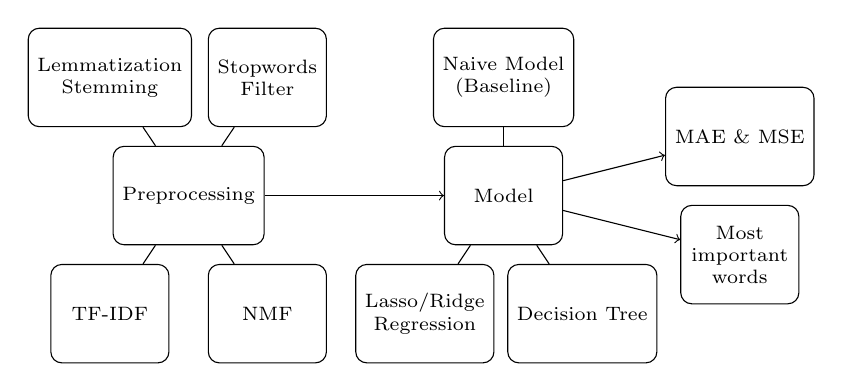
\begin{tikzpicture}[minimum width=1.5cm, minimum height=1.25cm, font=\scriptsize]
      \node[draw, align=center, rounded corners]  (P)   at ( 0,    0)    {Preprocessing};
      \node[draw, align=center, rounded corners]  (LS)  at (-1,  1.5)    {Lemmatization \\ Stemming};
      \node[draw, align=center, rounded corners]  (SF)  at ( 1,  1.5)    {Stopwords \\ Filter};
      \node[draw, align=center, rounded corners]  (T)   at (-1, -1.5)    {TF-IDF};
      \node[draw, align=center, rounded corners]  (N)   at ( 1, -1.5)    {NMF};

      \node[draw, align=center, rounded corners]  (M)   at ( 4,    0)    {Model};
      \node[draw, align=center, rounded corners]  (NM)  at ( 4,  1.5)    {Naive Model \\ (Baseline)};
      \node[draw, align=center, rounded corners]  (LR)  at ( 3, -1.5)    {Lasso/Ridge \\ Regression};
      \node[draw, align=center, rounded corners]  (D)   at ( 5, -1.5)    {Decision Tree};

      \node[draw, align=center, rounded corners]  (E)   at ( 7,  0.75)   {MAE \& MSE};
      \node[draw, align=center, rounded corners]  (W)   at ( 7, -0.75)   {Most \\ important \\ words};

      \draw[->] (P) -- (M);

      \draw[-] (P) -- (LS);
      \draw[-] (P) -- (SF);
      \draw[-] (P) -- (T);
      \draw[-] (P) -- (N);

      \draw[-] (M) -- (NM);
      \draw[-] (M) -- (LR);
      \draw[-] (M) -- (D);

      \draw[->] (M) -- (E);
      \draw[->] (M) -- (W);
    \end{tikzpicture}
    \label{flowchart}
    \caption{Flowchart for our methods.}
  \end{figure}

  We test the model in two approaches:

  \begin{itemize}
    \item Split the data from some years into training dataset (80\%) and test dataset (20\%), and repeat the experiment to avoid flukes;
    \item Train the model via the data from some years and forecast the following year.
  \end{itemize}

\end{frame}

\section{Result}

\begin{frame}{Result - Error}

  \begin{figure}[H]
    \centering
    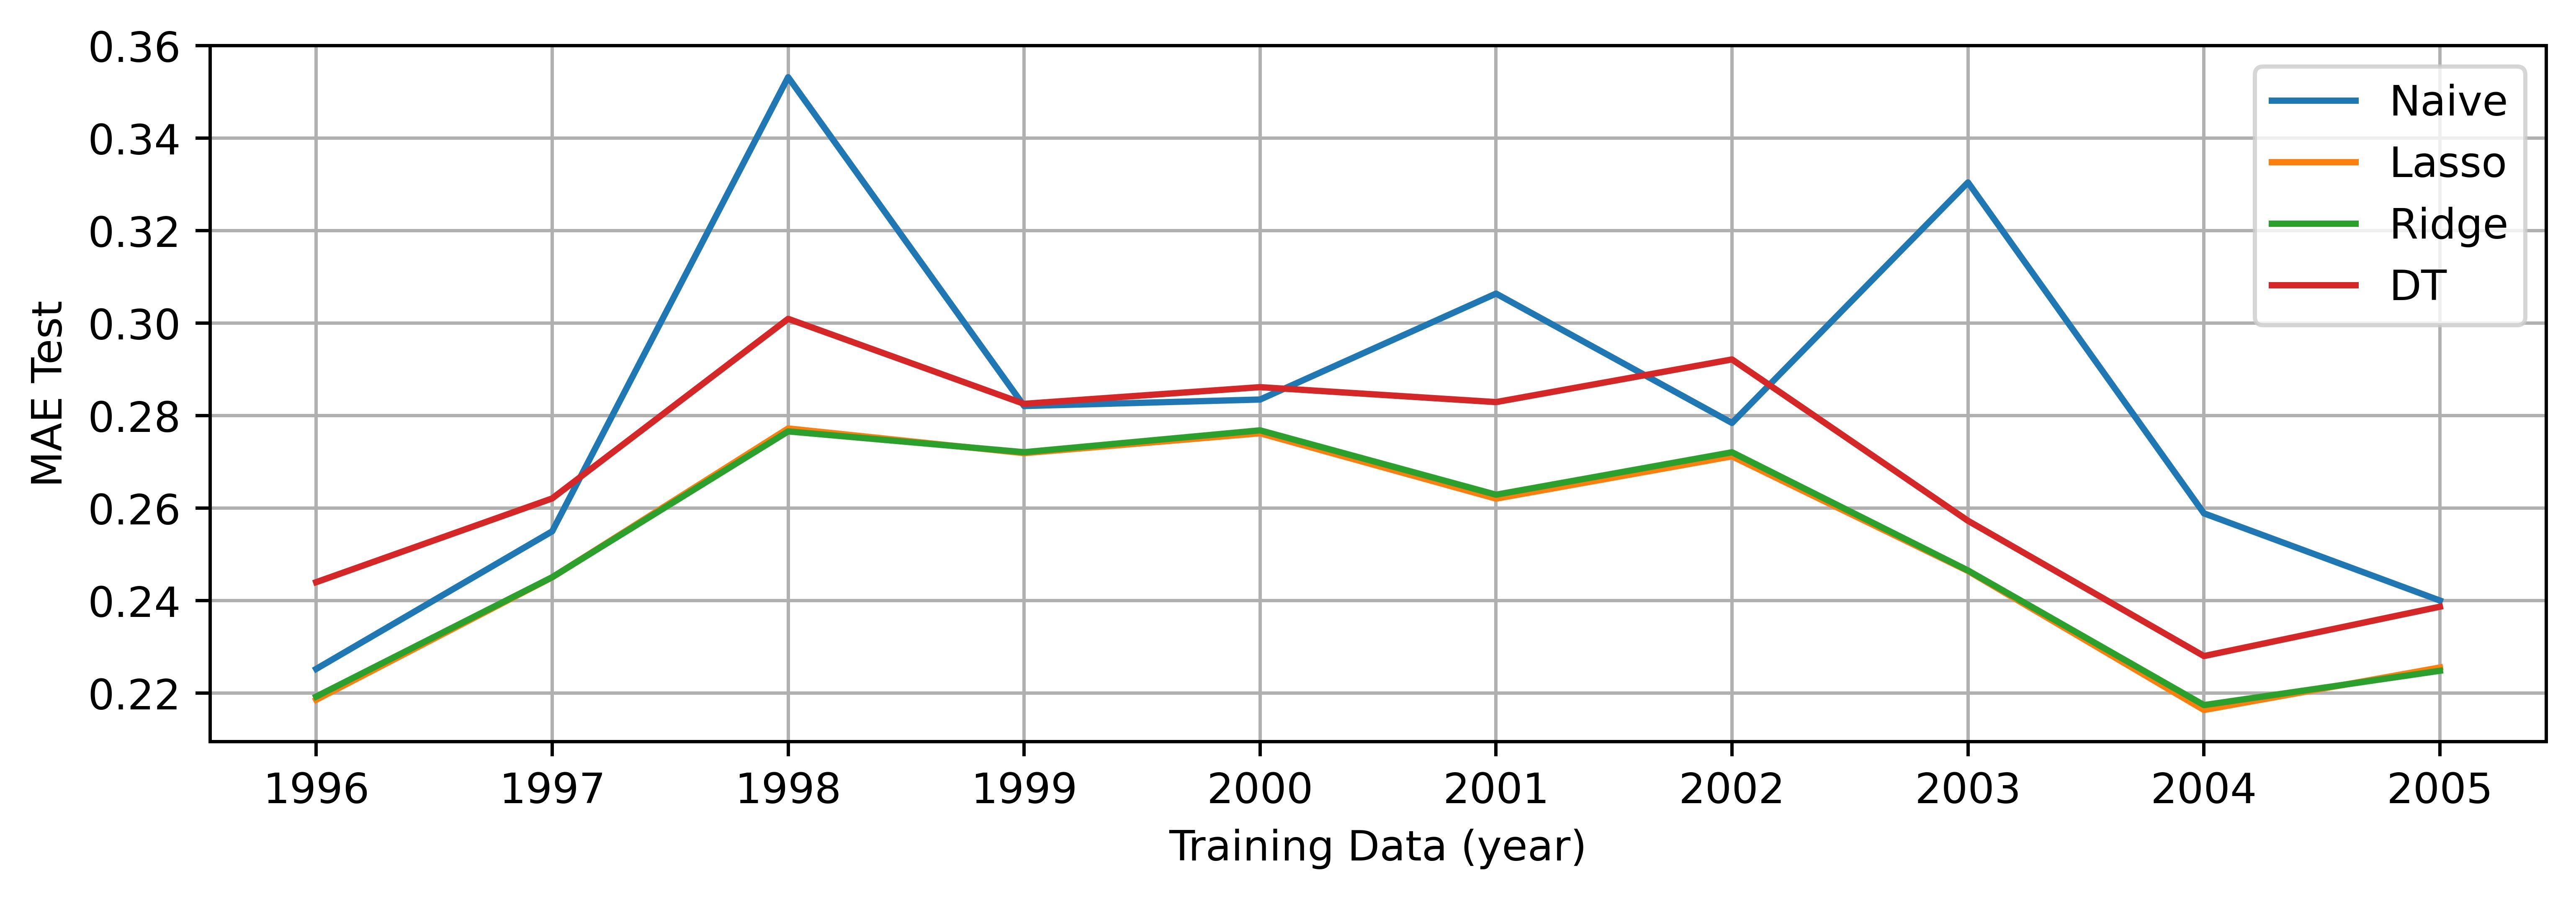
\includegraphics[width=0.7\textwidth]{../Result/Res-1_MAE_test.jpg} \\
    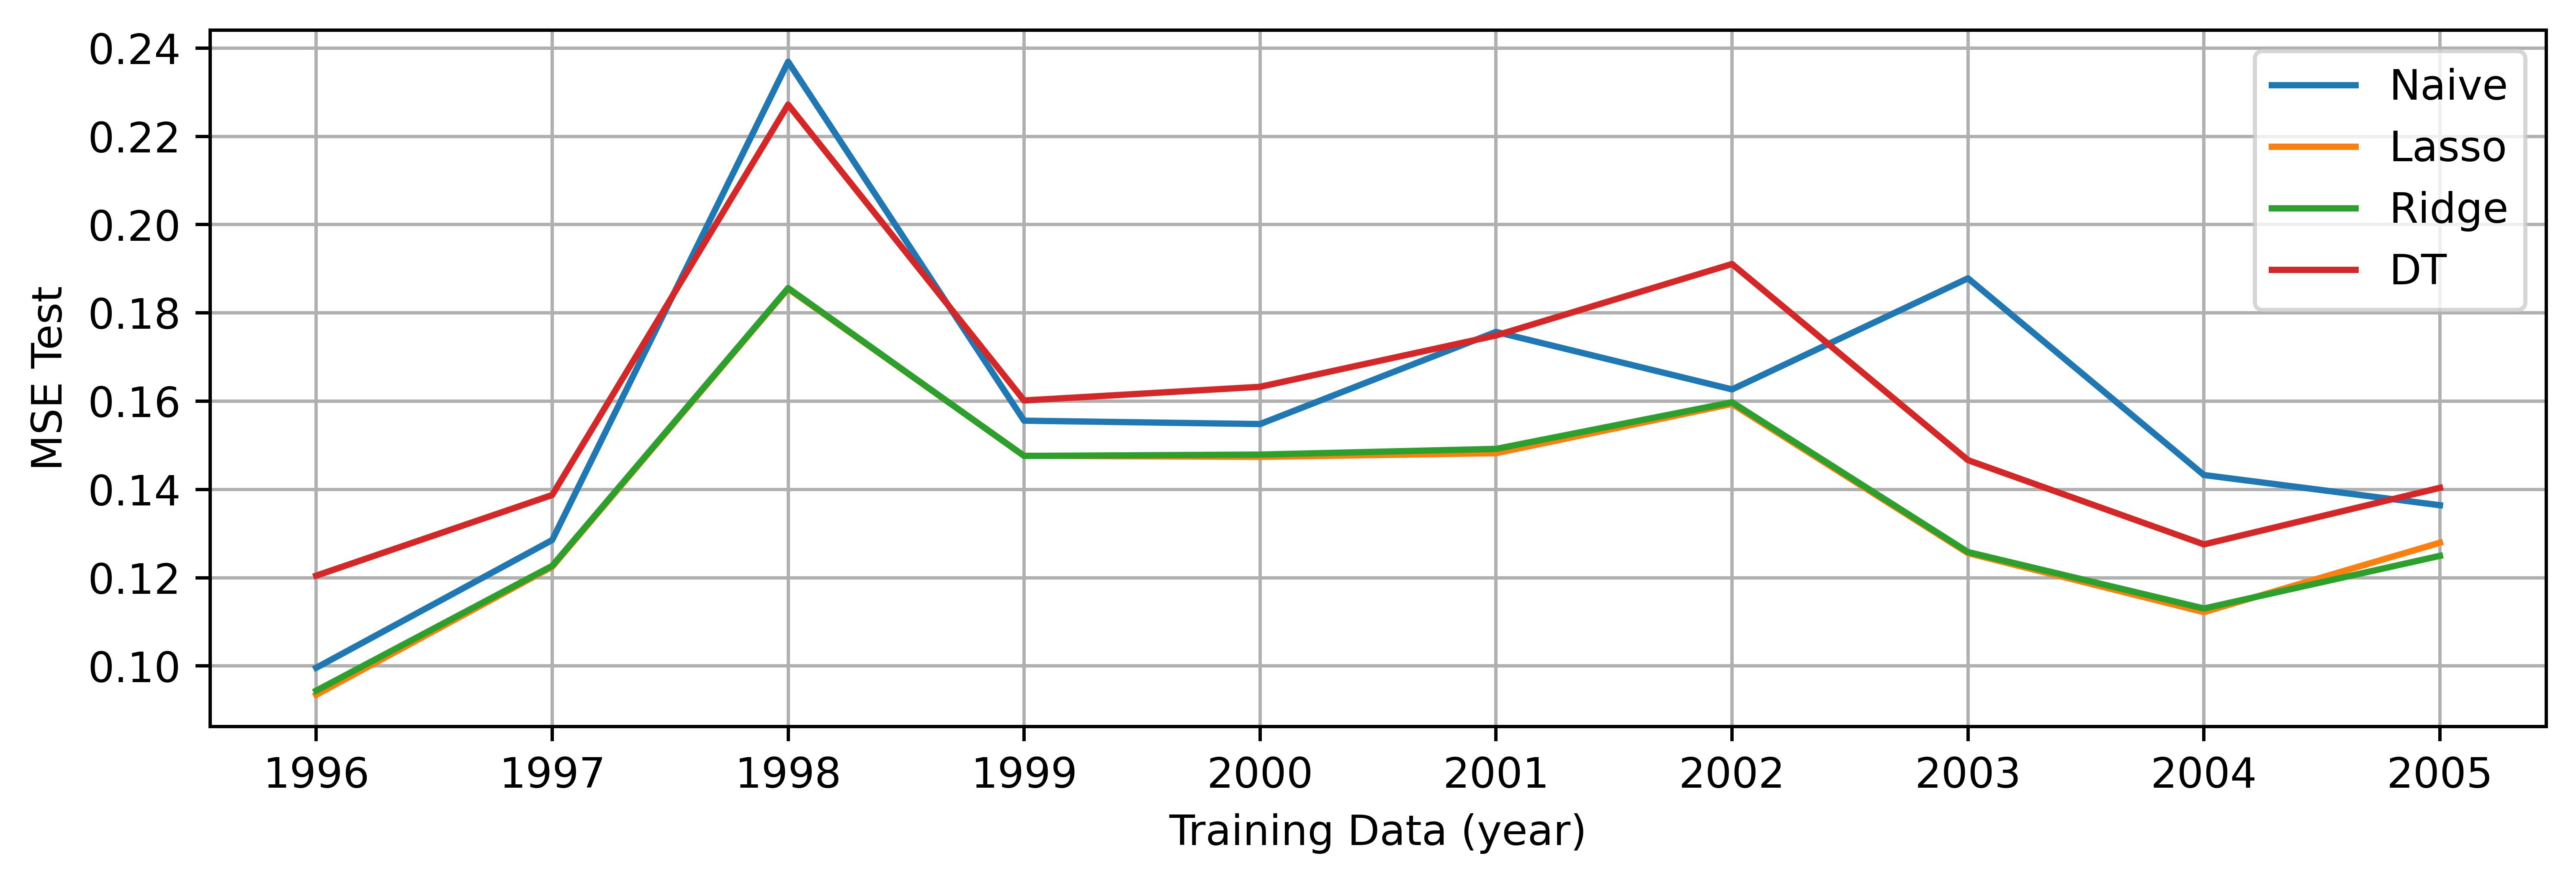
\includegraphics[width=0.7\textwidth]{../Result/Res-1_MSE_test.jpg}
    \caption{MAE and MSE for testing 1-year training set.}
  \end{figure}

\end{frame}

\begin{frame}{Result - Error}

  \begin{figure}[H]
    \centering
    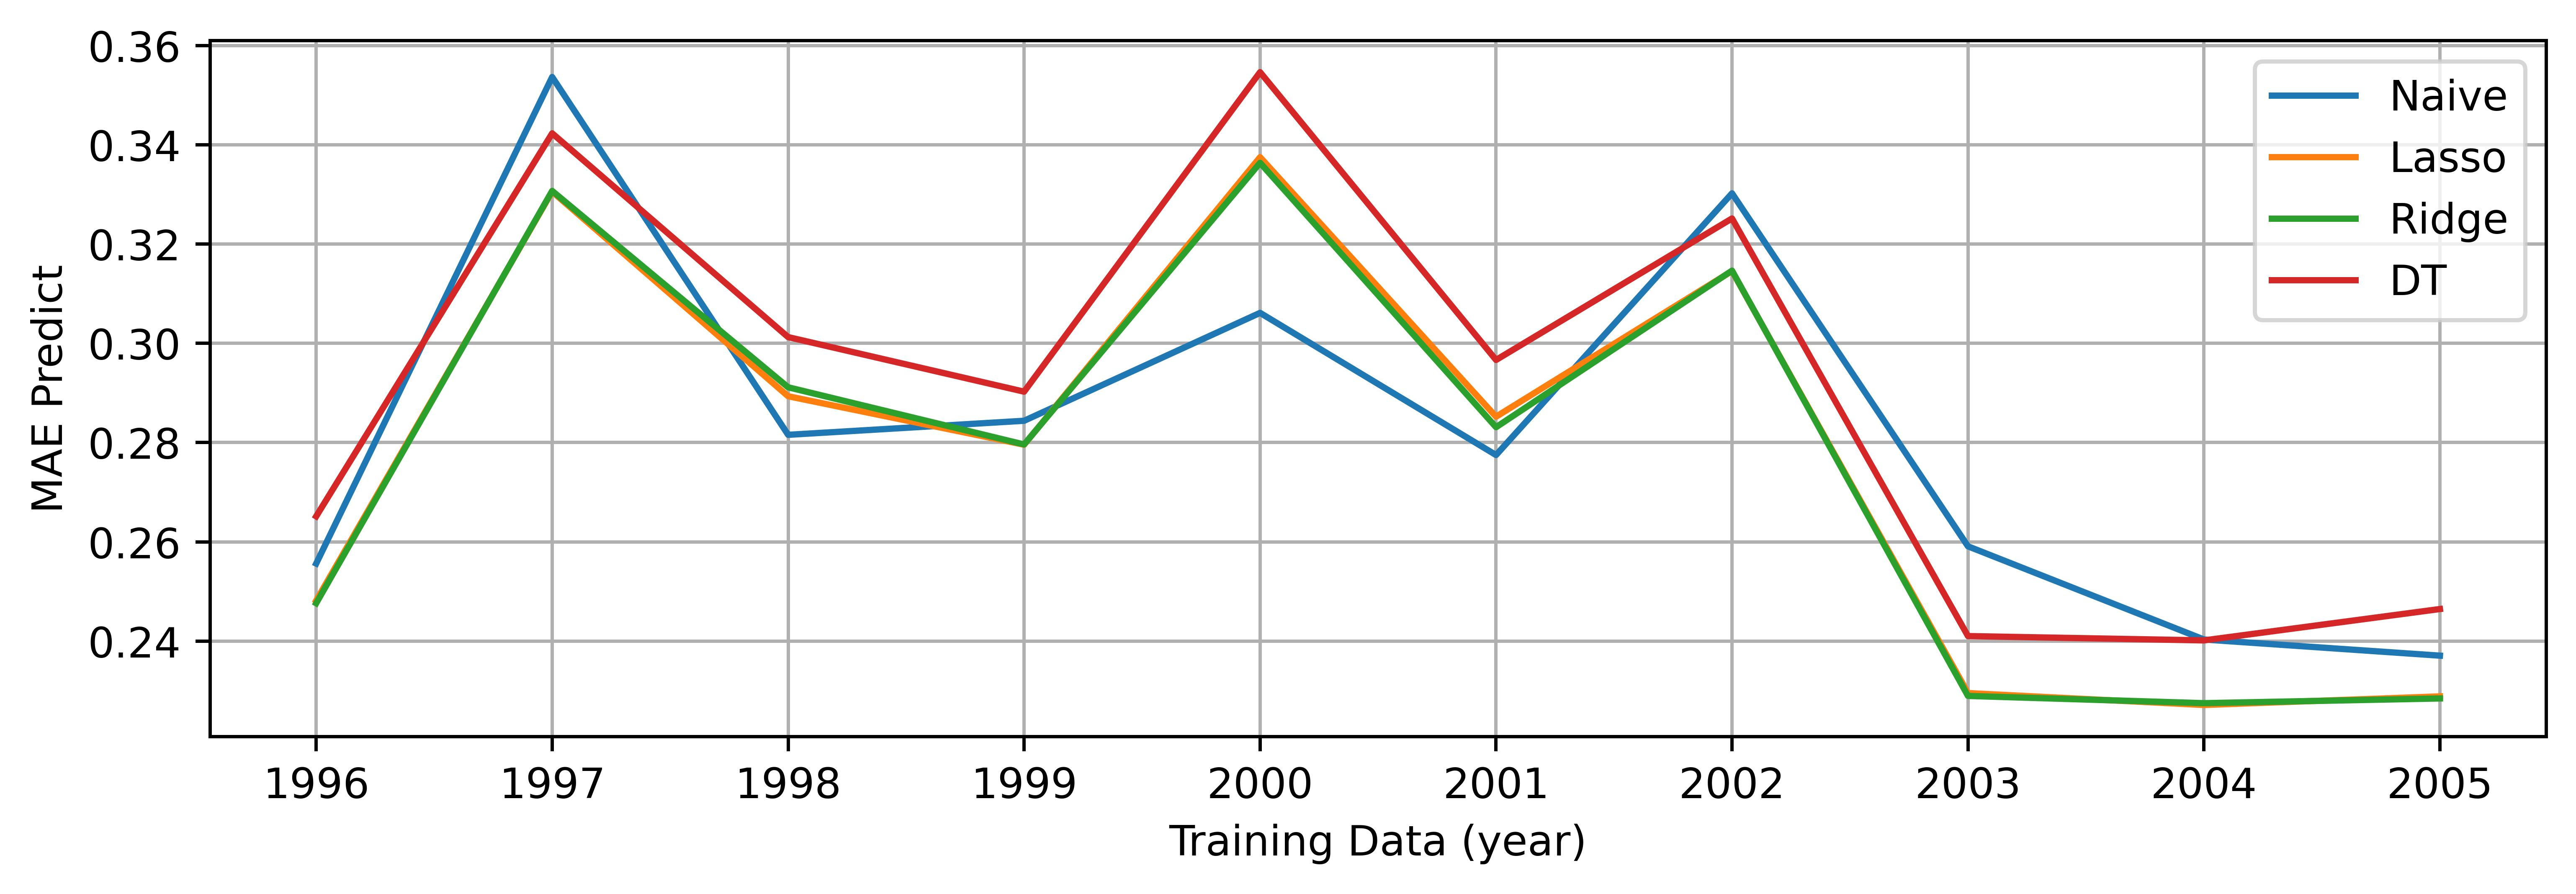
\includegraphics[width=0.7\textwidth]{../Result/Res-1_MAE_pred.jpg} \\
    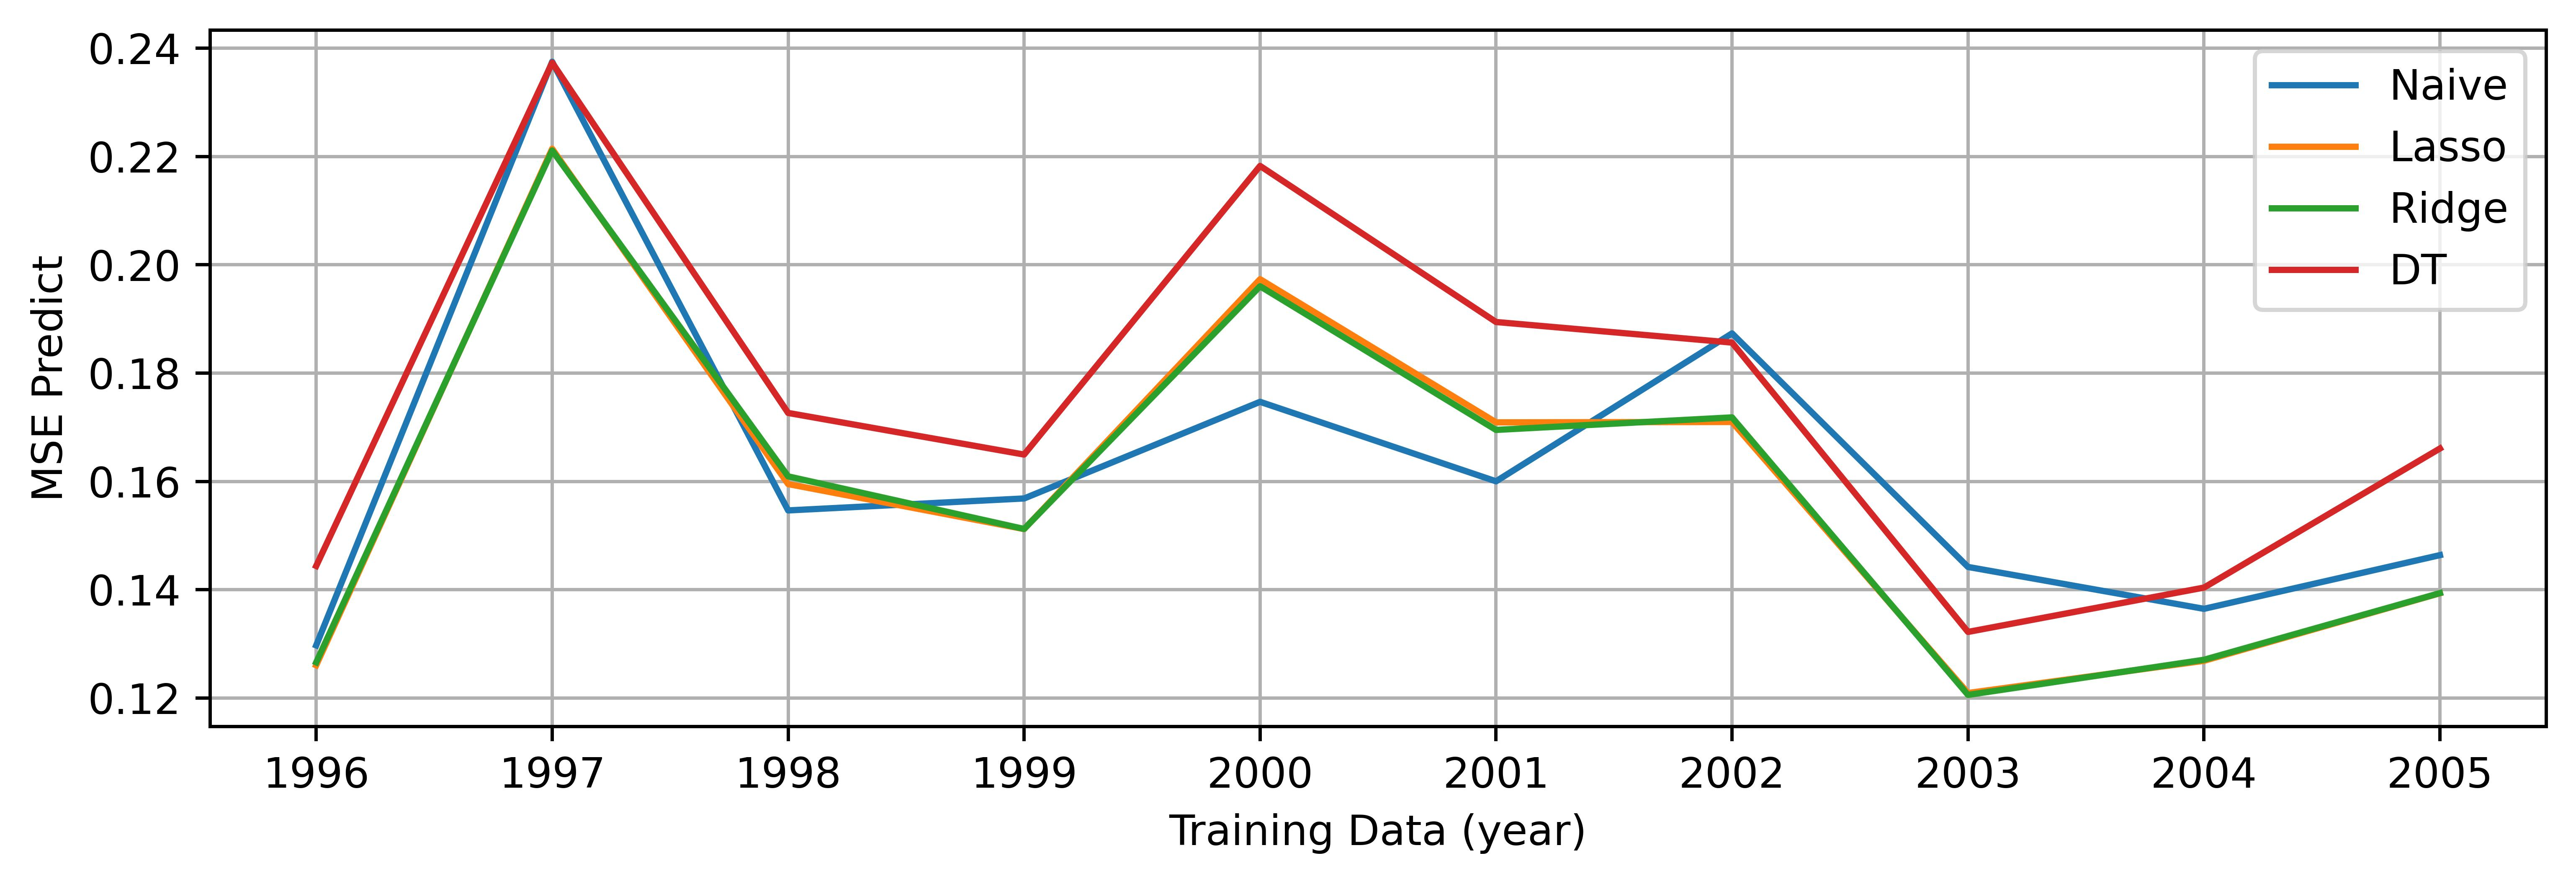
\includegraphics[width=0.7\textwidth]{../Result/Res-1_MSE_pred.jpg}
    \caption{MAE and MSE for predicting 1-year training set.}
  \end{figure}

\end{frame}

\begin{frame}{Result - Error}

  \begin{figure}[H]
    \centering
    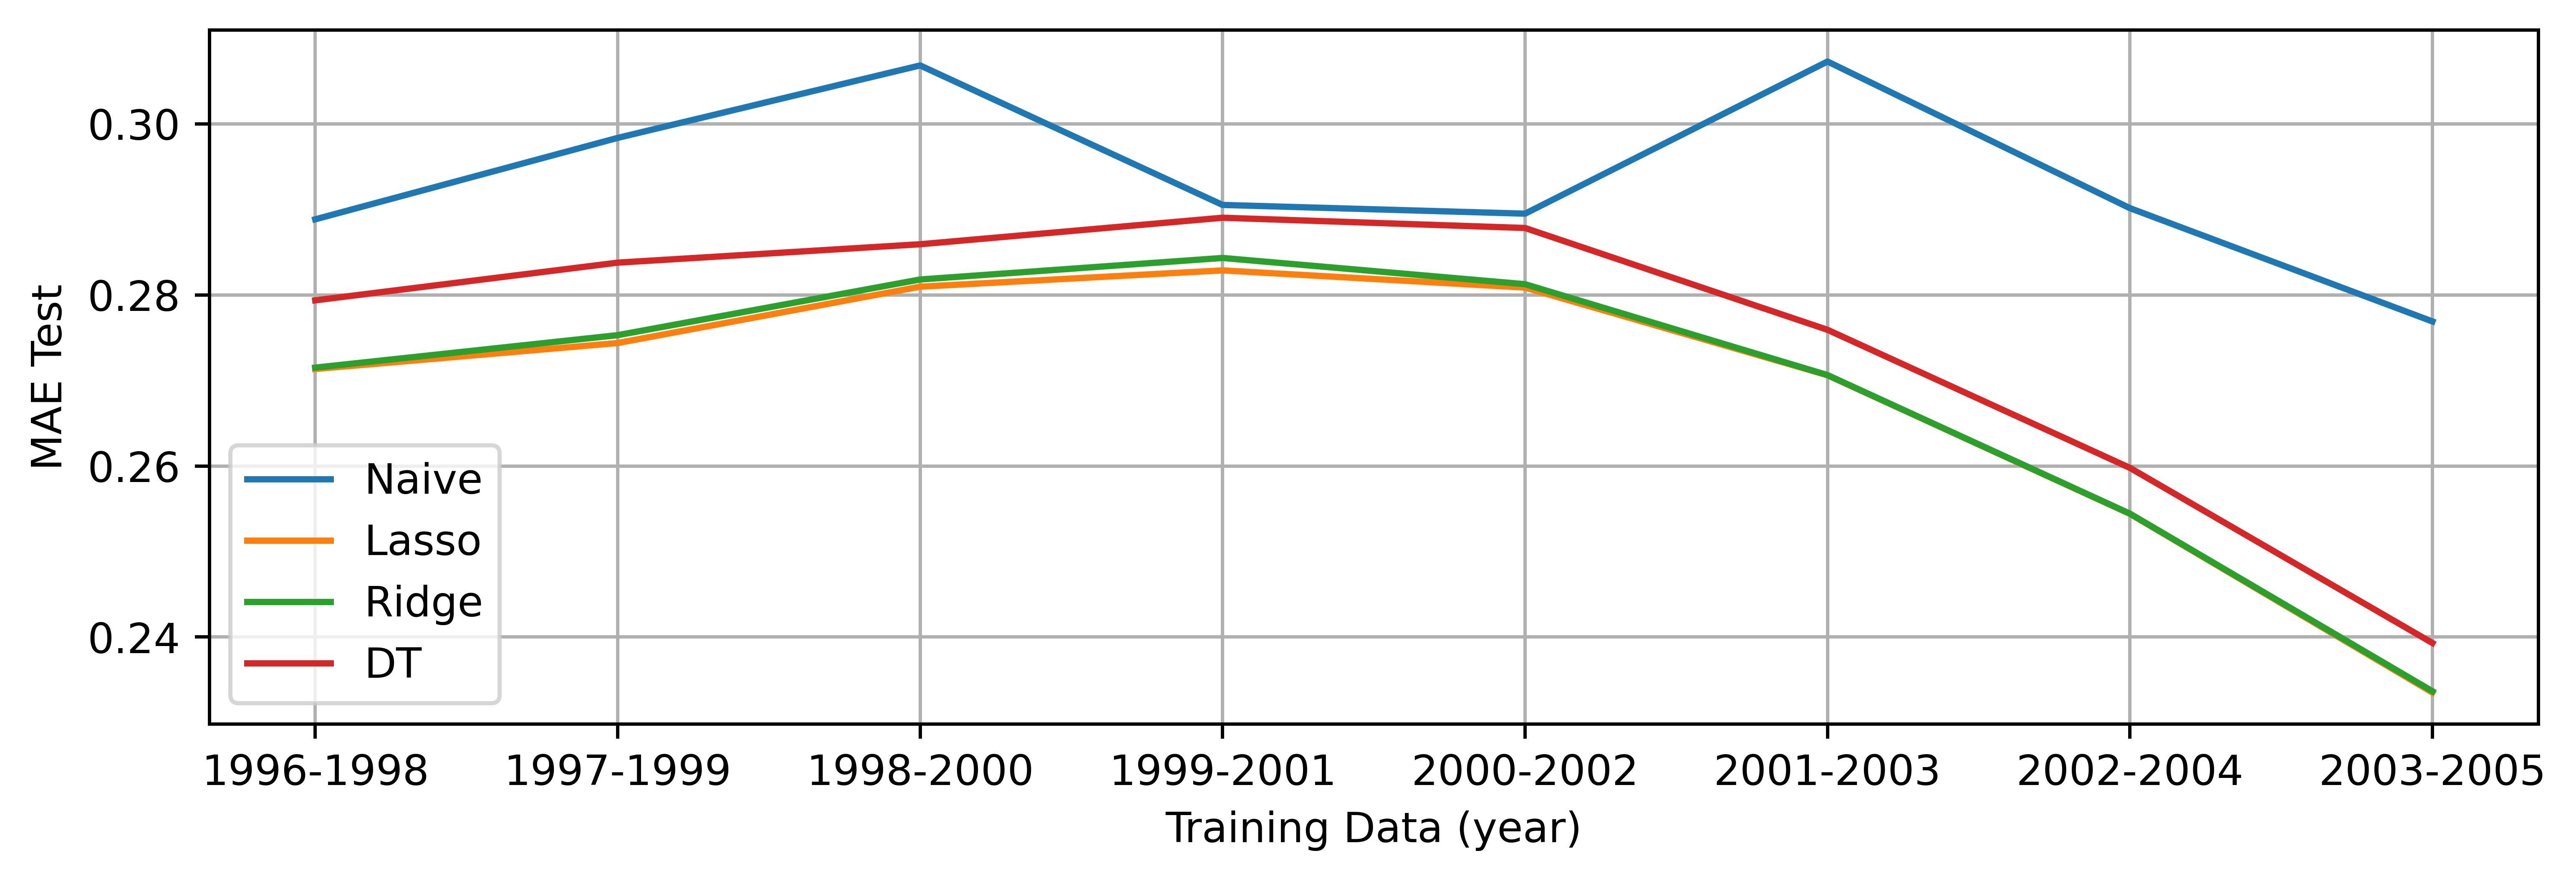
\includegraphics[width=0.7\textwidth]{../Result/Res-3_MAE_test.jpg} \\
    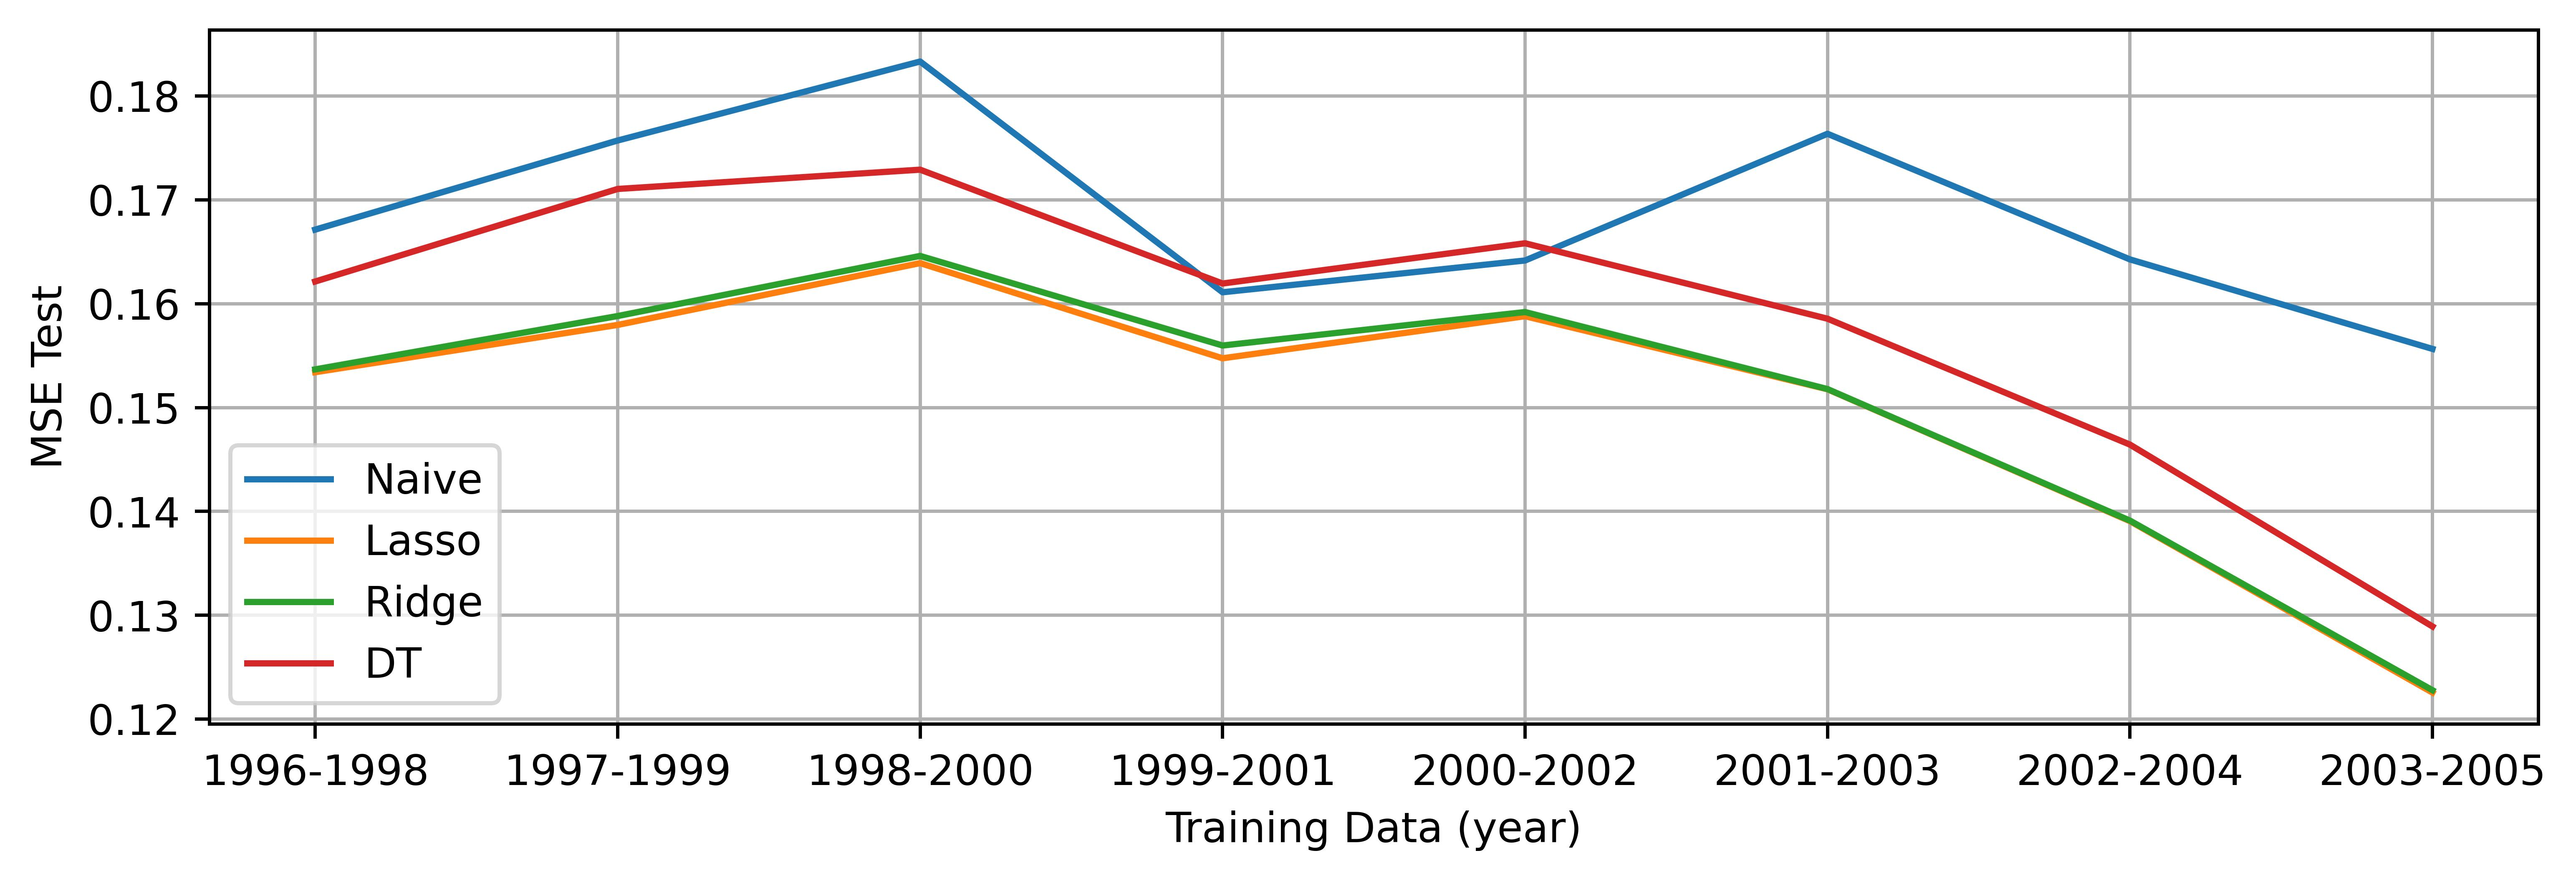
\includegraphics[width=0.7\textwidth]{../Result/Res-3_MSE_test.jpg}
    \caption{MAE and MSE for testing 3-year training set.}
  \end{figure}

\end{frame}

\begin{frame}{Result - Error}

  \begin{figure}[H]
    \centering
    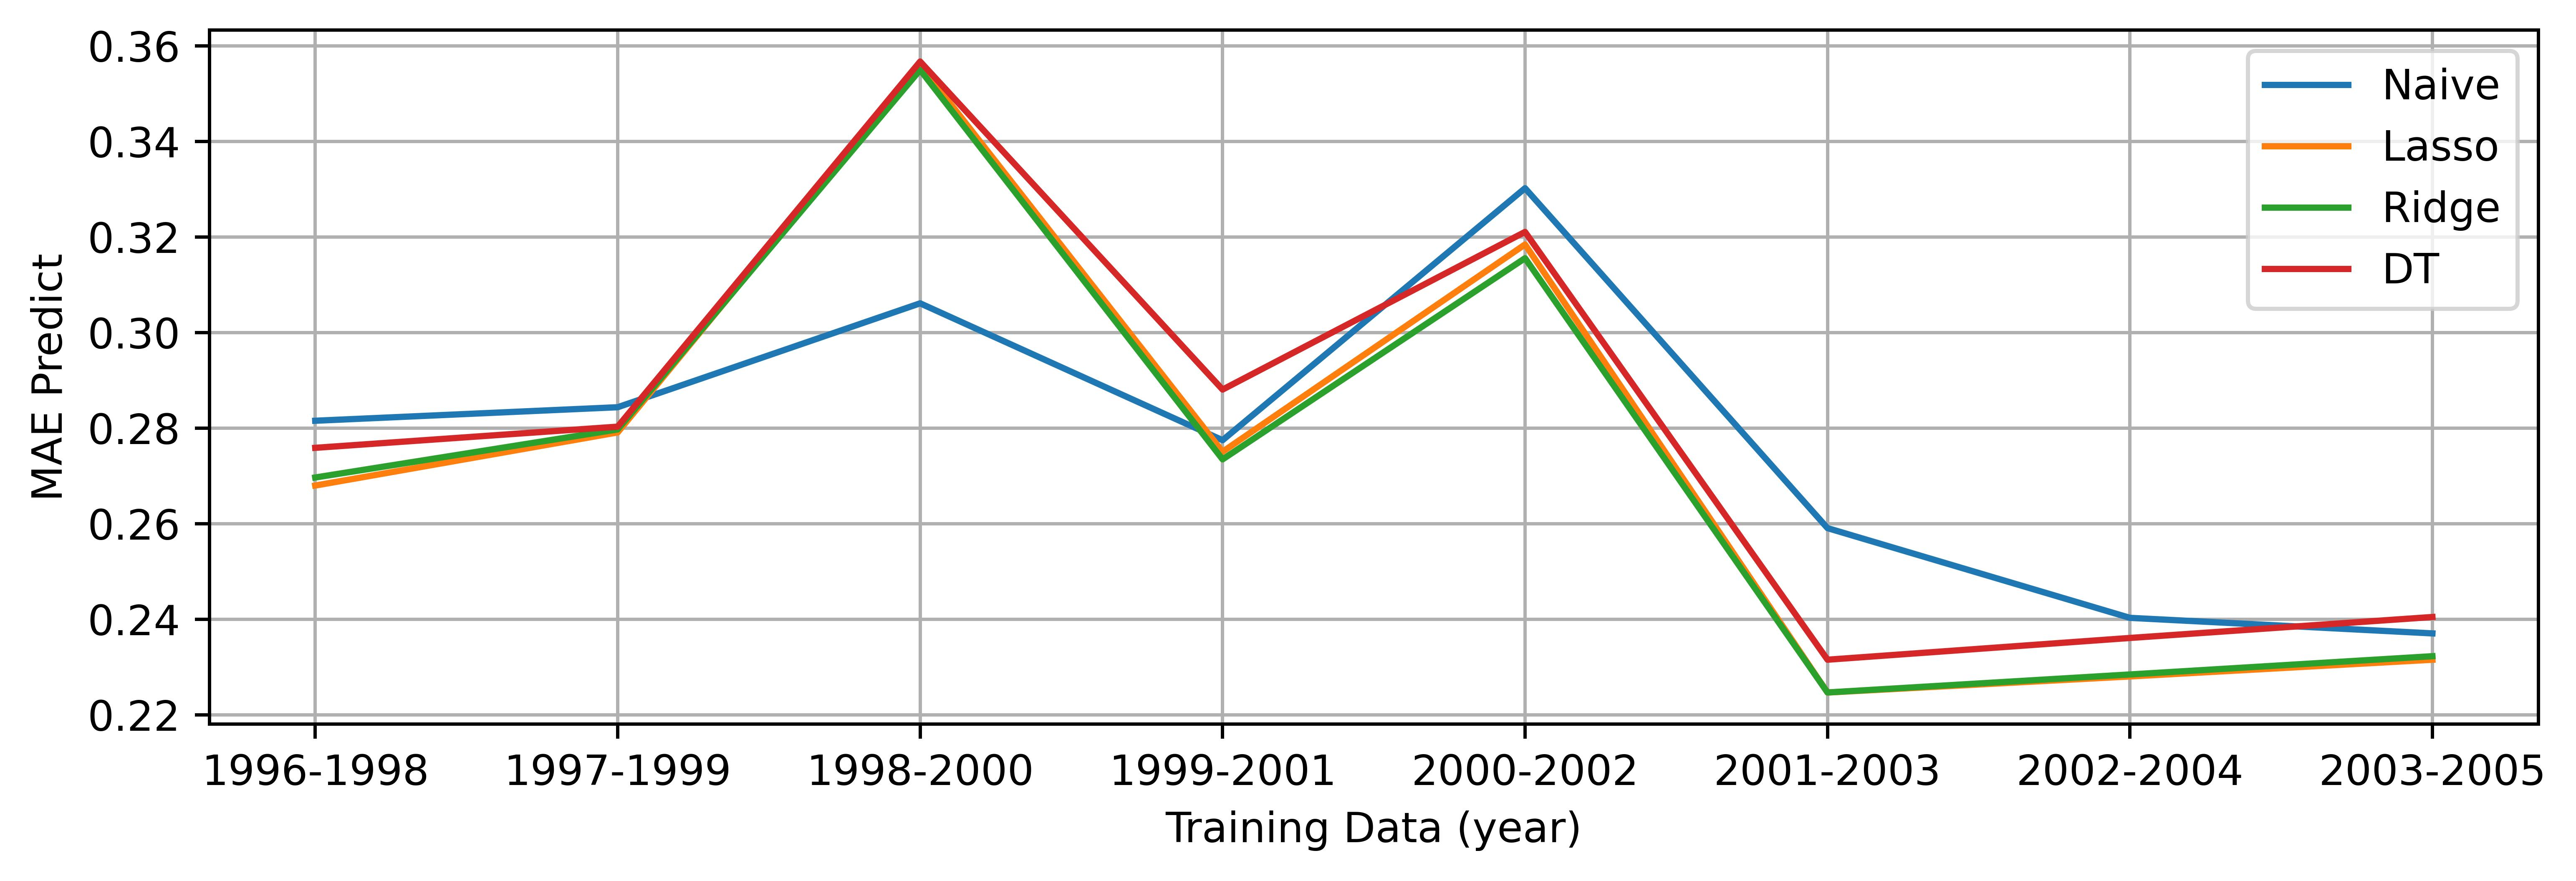
\includegraphics[width=0.7\textwidth]{../Result/Res-3_MAE_pred.jpg} \\
    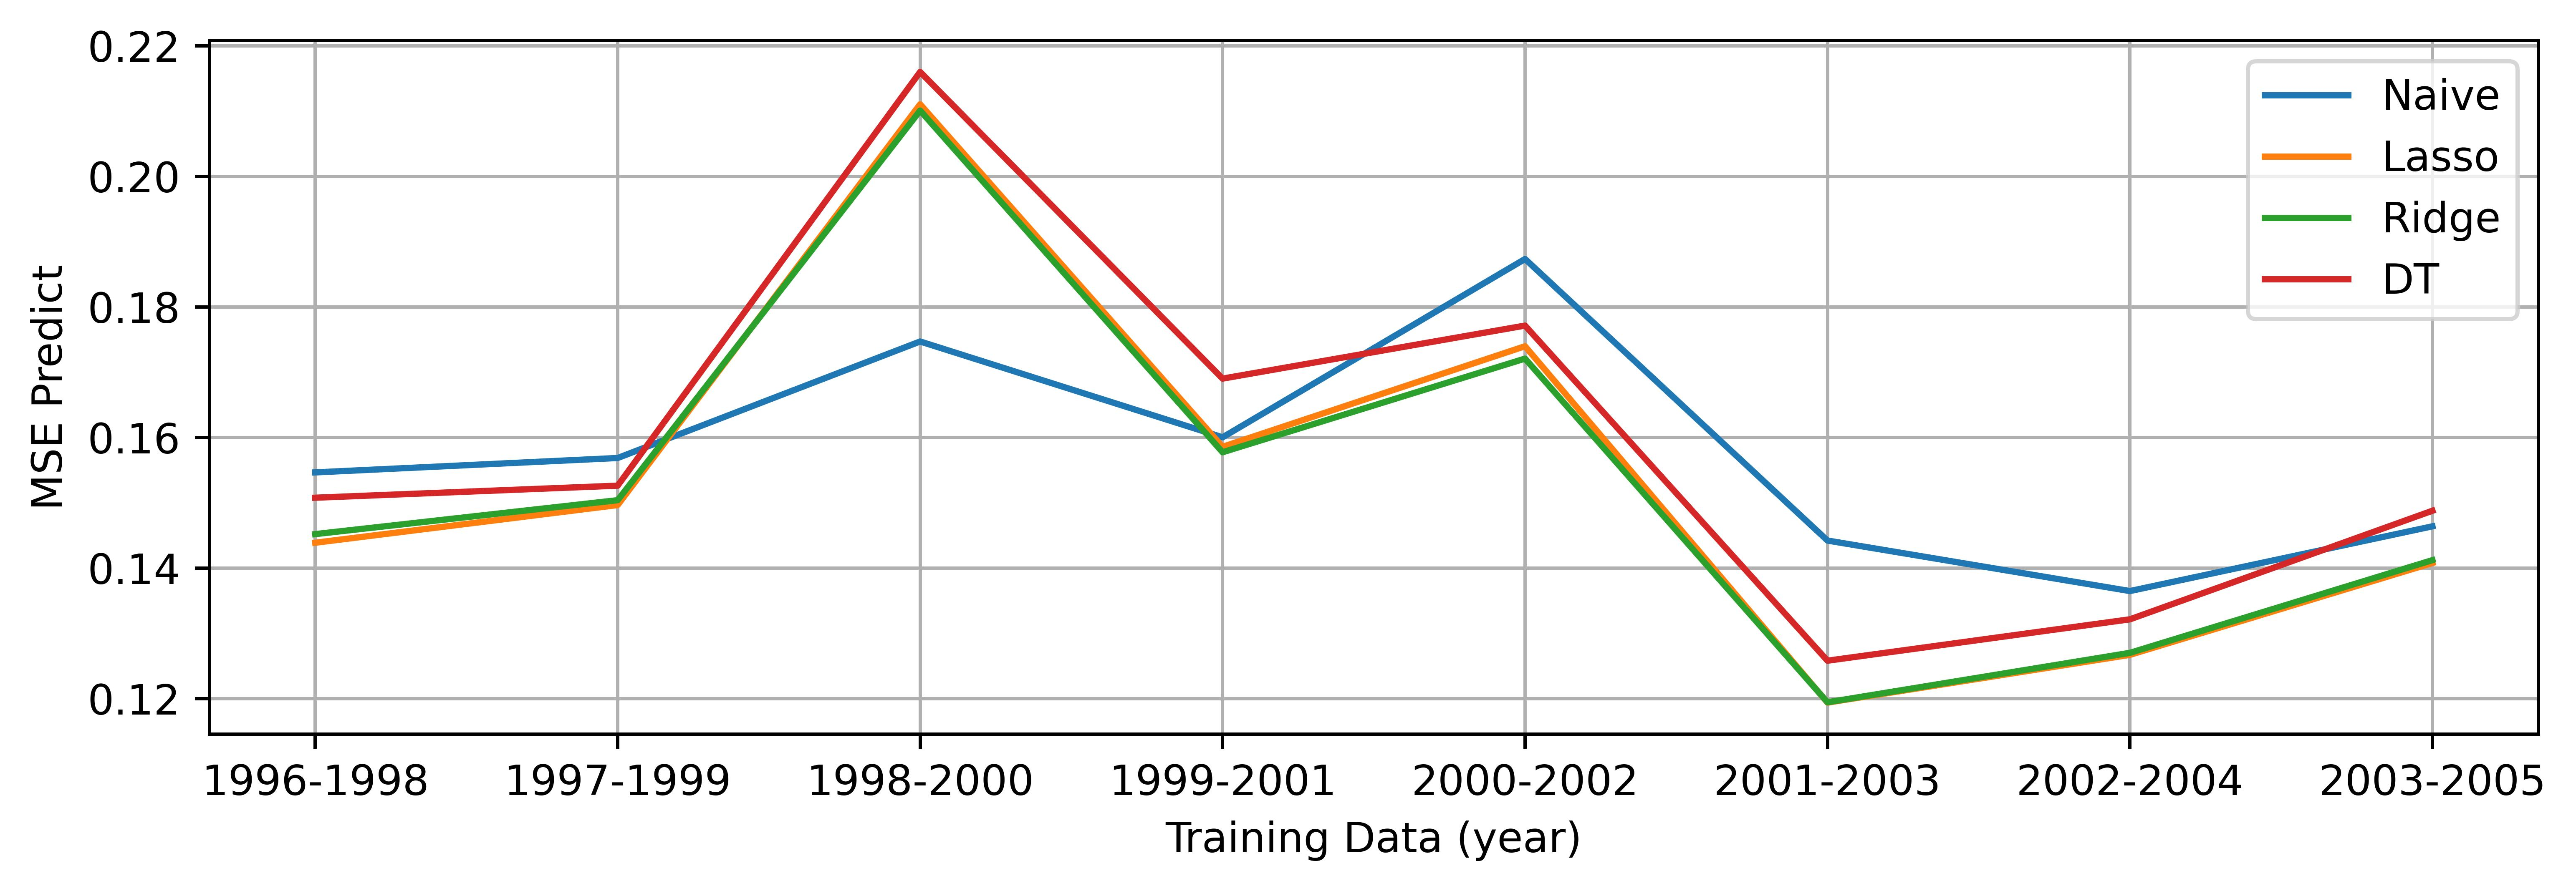
\includegraphics[width=0.7\textwidth]{../Result/Res-3_MSE_pred.jpg}
    \caption{MAE and MSE for predicting 3-year training set.}
  \end{figure}

\end{frame}

\begin{frame}{Result - Word Features}

  \begin{table}[H]
    \centering
    \begin{tabular}{|c|c|c|c|}
      \hline
      Year      & Increasing Common & Decreasing Common & Different \\
      \hline
      1996-1997 & $21.0\%$          & $70.0\%$          & $0.0\%$   \\
      \hline
      1997-1998 & $27.0\%$          & $13.0\%$          & $0.5\%$   \\
      \hline
      1998-1999 & $1.0\%$           & $43.0\%$          & $1.5\%$   \\
      \hline
      1999-2000 & $3.0\%$           & $5.0\%$           & $0.5\%$   \\
      \hline
      2000-2001 & $3.0\%$           & $2.0\%$           & $0.5\%$   \\
      \hline
      2001-2002 & $1.0\%$           & $25.0\%$          & $1.0\%$   \\
      \hline
      2002-2003 & $52.0\%$          & $33.0\%$          & $0.0\%$   \\
      \hline
      2003-2004 & $0.0\%$           & $4.0\%$           & $2.5\%$   \\
      \hline
      2004-2005 & $29.0\%$          & $50.0\%$          & $0.5\%$   \\
      \hline
    \end{tabular}
    \caption{Word features for lasso regression between different years.}
  \end{table}

\end{frame}

\begin{frame}{Result - Word Features}

  \begin{table}[H]
    \centering
    \begin{tabular}{|c|c|c|c|}
      \hline
      Year      & Increasing Common & Decreasing Common & Different \\
      \hline
      1996-1997 & $11.0\%$          & $54.0\%$          & $2.5\%$   \\
      \hline
      1997-1998 & $29.0\%$          & $45.0\%$          & $0.5\%$   \\
      \hline
      1998-1999 & $0.0\%$           & $27.0\%$          & $11.5\%$  \\
      \hline
      1999-2000 & $0.0\%$           & $67.0\%$          & $0.5\%$   \\
      \hline
      2000-2001 & $2.0\%$           & $20.0\%$          & $0.5\%$   \\
      \hline
      2001-2002 & $29.0\%$          & $25.0\%$          & $1.0\%$   \\
      \hline
      2002-2003 & $24.0\%$          & $34.0\%$          & $12.5\%$  \\
      \hline
      2003-2004 & $2.0\%$           & $62.0\%$          & $0.5\%$   \\
      \hline
      2004-2005 & $34.0\%$          & $25.0\%$          & $2.5\%$   \\
      \hline
    \end{tabular}
    \caption{Word features for ridge regression between different years.}
  \end{table}

\end{frame}

\begin{frame}{Result - Word Features}

  \begin{table}[H]
    \centering
    \begin{tabular}{|c|c|c|c|}
      \hline
      Year      & Increasing Common & Decreasing Common & Different \\
      \hline
      1996-1997 & $67.0\%$          & $9.0\%$           & $0.0\%$   \\
      \hline
      1997-1998 & $74.0\%$          & $11.0\%$          & $0.0\%$   \\
      \hline
      1998-1999 & $64.0\%$          & $24.0\%$          & $0.0\%$   \\
      \hline
      1999-2000 & $67.0\%$          & $10.0\%$          & $0.0\%$   \\
      \hline
      2000-2001 & $71.0\%$          & $32.0\%$          & $0.0\%$   \\
      \hline
      2001-2002 & $62.0\%$          & $8.0\%$           & $0.0\%$   \\
      \hline
      2002-2003 & $56.0\%$          & $8.0\%$           & $0.0\%$   \\
      \hline
      2003-2004 & $72.0\%$          & $15.0\%$          & $0.0\%$   \\
      \hline
      2004-2005 & $77.0\%$          & $35.0\%$          & $0.0\%$   \\
      \hline
    \end{tabular}
    \caption{Word features for decision tree between different years.}
  \end{table}

\end{frame}

\begin{frame}{Result - Word Features}

  \begin{table}[H]
    \centering
    \begin{tabular}{|c|c|c|c|}
      \hline
      Year & Lasso Ridge               & Lasso DT                  & Ridge DT                  \\
      \hline
      1996 & $68.0\%$/$91.0\%$/$0.0\%$ & $8.0\%$/$0.0\%$/$19.0\%$  & $6.0\%$/$0.0\%$/$23.5\%$  \\
      \hline
      1997 & $62.0\%$/$76.0\%$/$0.5\%$ & $27.0\%$/$0.0\%$/$18.5\%$ & $39.0\%$/$0.0\%$/$15.5\%$ \\
      \hline
      1998 & $91.0\%$/$62.0\%$/$0.0\%$ & $33.0\%$/$0.0\%$/$8.0\%$  & $36.0\%$/$0.0\%$/$13.5\%$ \\
      \hline
      1999 & $19.0\%$/$23.0\%$/$2.5\%$ & $6.0\%$/$0.0\%$/$13.5\%$  & $7.0\%$/$0.0\%$/$34.0\%$  \\
      \hline
      2000 & $35.0\%$/$18.0\%$/$2.5\%$ & $18.0\%$/$0.0\%$/$5.5\%$  & $11.0\%$/$0.0\%$/$33.5\%$ \\
      \hline
      2001 & $22.0\%$/$74.0\%$/$1.5\%$ & $7.0\%$/$0.0\%$/$19.0\%$  & $34.0\%$/$0.0\%$/$17.0\%$ \\
      \hline
      2002 & $95.0\%$/$90.0\%$/$0.0\%$ & $24.0\%$/$0.0\%$/$16.0\%$ & $26.0\%$/$0.0\%$/$19.0\%$ \\
      \hline
      2003 & $59.0\%$/$24.0\%$/$2.5\%$ & $22.0\%$/$0.0\%$/$6.5\%$  & $16.0\%$/$0.0\%$/$34.0\%$ \\
      \hline
      2004 & $56.0\%$/$49.0\%$/$0.5\%$ & $8.0\%$/$0.0\%$/$21.0\%$  & $13.0\%$/$0.0\%$/$27.0\%$ \\
      \hline
      2005 & $76.0\%$/$73.0\%$/$0.0\%$ & $24.0\%$/$0.0\%$/$11.5\%$ & $23.0\%$/$0.0\%$/$22.0\%$ \\
      \hline
    \end{tabular}
    \caption{Word features between different models (Increasing Common, Decreasing Common, Different).}
  \end{table}

\end{frame}

\section{Conclusion}

\begin{frame}{Conclusion}

  For forecasting, similar to the previous research \footfullcite{kogan2009predicting}:

  \begin{itemize}
    \item More training data can lead to higher accuracy and stablity; \vspace{.25cm}
    \item The Sarbanes–Oxley Act (2002) changes the information/distribution of the words in text; \vspace{.25cm}
    \item The Sarbanes–Oxley Act (2002) makes a higher accuracy in prediction.
  \end{itemize}

\end{frame}

\begin{frame}{Conclusion}

  For the words features: \vspace{.25cm}

  \begin{itemize}
    \item There exists the similarity between different years; \vspace{.25cm}
    \item The lasso/ridge regression can give the same features; \vspace{.25cm}
    \item The decision tree always choose the same feature, but it seems not good; \vspace{.25cm}
    \item Compare with the features of increasing, the of features decreasing are more similar between years.
  \end{itemize}

\end{frame}

\section*{Reference}
\begin{frame}[allowframebreaks]{Reference}
  \printbibliography
\end{frame}

\appendix

\end{document}